\documentclass[border=7pt]{standalone}

\usepackage{pgfplots}
\usepackage{xcolor}
\pgfplotsset{compat=newest}

\newcommand{\DrawSurfacePlot}{%
    \addplot3[
      surf,
      fill opacity=0.7,
      color=teal!80!black,
      faceted color=blue!80!black,
      line width=1pt,
      domain=-2.5:2.5
    ] {2*x*y - 1};%
}

\begin{document}

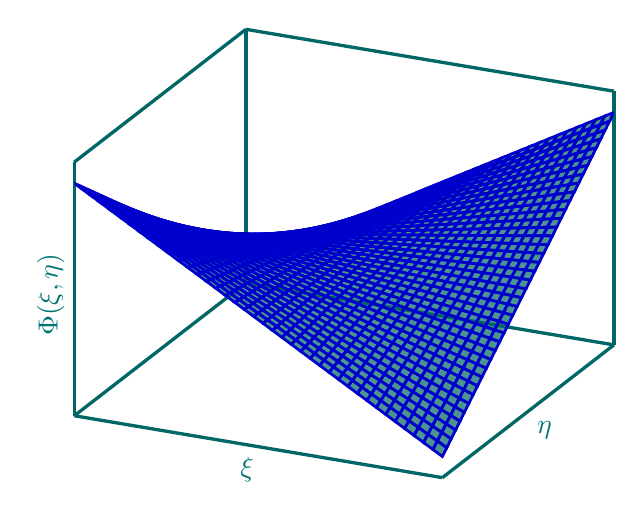
\begin{tikzpicture}
  \begin{axis}[
    samples=40, 
    ticks=none,
    xlabel={$\xi$},
    ylabel={$\eta$},
    zlabel={$\Phi(\xi,\eta)$},
    axis line style={very thick, teal!80!black},
    label style={font=\bfseries\color{teal!90!black}},
  ]

\DrawSurfacePlot
    
  \end{axis}
\end{tikzpicture}

\end{document}
